%%=============================================================================
%% resultaten vergelijkend onderzoek
%%=============================================================================

\chapter{Resultaten vergelijkend onderzoek}
\label{ch:Resultaten vergelijkend onderzoek}
Wie in detail wilt bekijken hoe de resultaten zijn bekomen, kan meer informatie vinden bij \ref{appendix:stappenplan analyse}.

\section{Vergelijking van de assistenten in spraakkwaliteit}
\label{s:Vergelijking van de assistenten in spraakkwaliteit}

\subsection{Vergelijking van de assistenten per eigenschap}
\label{ss:Vergelijking van de assistenten per eigenschap}

\begin{figure}[h]
    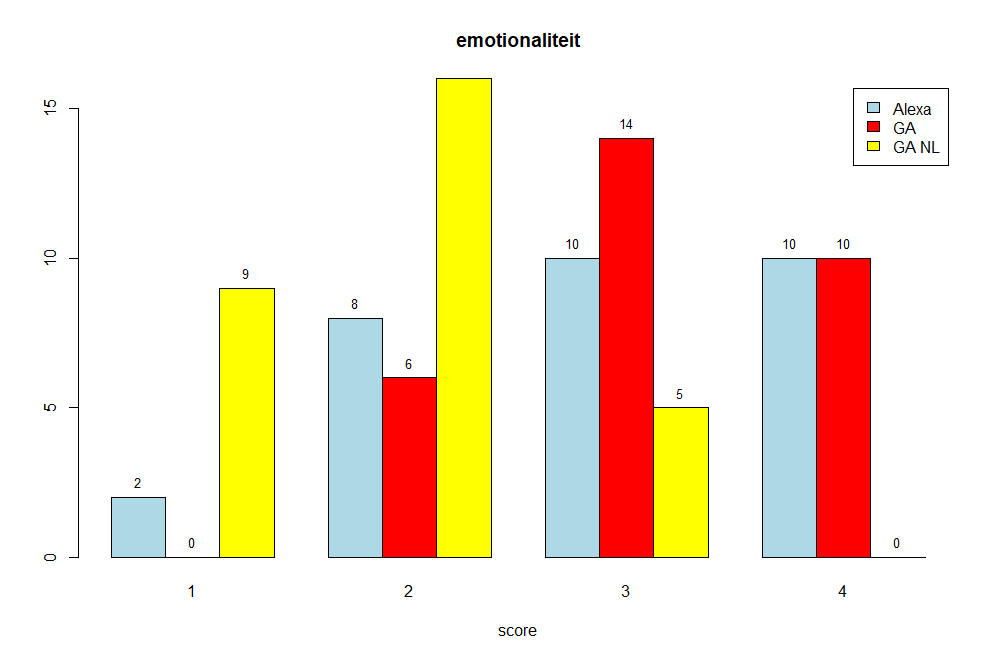
\includegraphics[width=0.9\linewidth]{../onderzoek/onderzoeksresultaten/vergelijking_assistenten_per_eigenschap/barplot/barplot_score_emotionaliteit}
    \caption{De score die de deelnemers hebben gegeven op de emotionaliteit van de assistenten}
    \label{fig:barplot-emotionaliteit}
\end{figure}

\begin{figure}[h]
    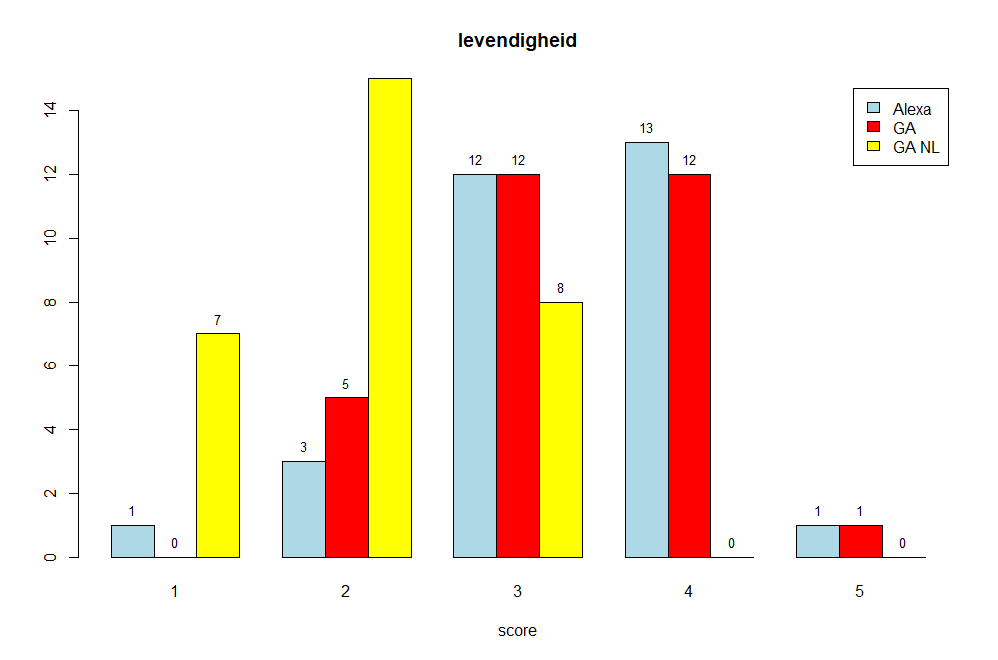
\includegraphics[width=0.9\linewidth]{../onderzoek/onderzoeksresultaten/vergelijking_assistenten_per_eigenschap/barplot/barplot_score_levendigheid}
    \caption{De score die de deelnemers hebben gegeven op de levendigheid van de assistenten}
    \label{fig:barplot-levendigheid}
\end{figure}

\begin{figure}[h]
    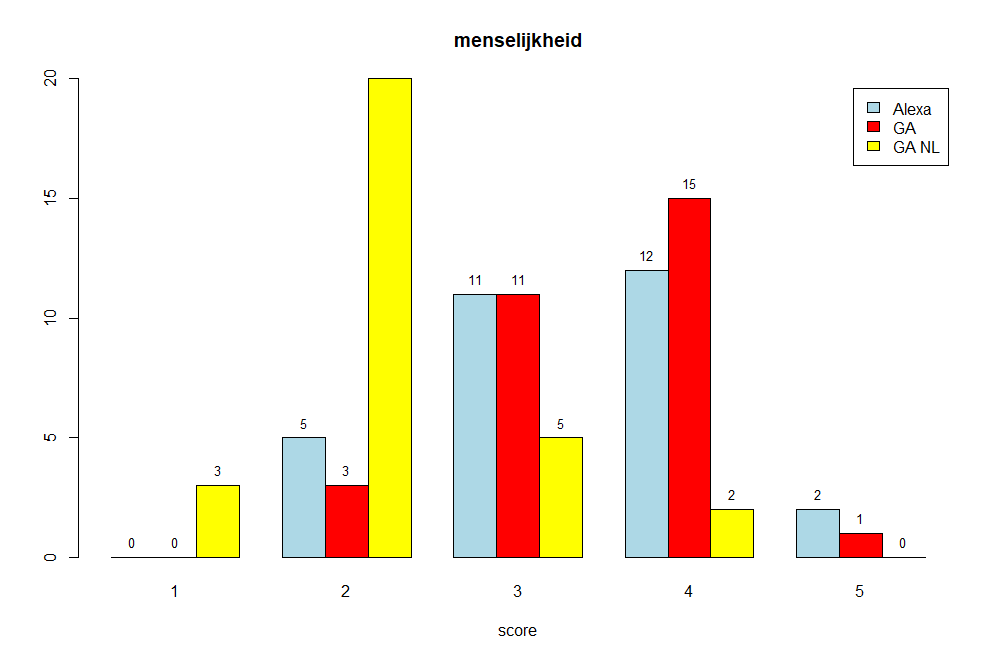
\includegraphics[width=0.9\linewidth]{../onderzoek/onderzoeksresultaten/vergelijking_assistenten_per_eigenschap/barplot/barplot_score_menselijkheid}
    \caption{De score die de deelnemers hebben gegeven op de menselijkheid van de assistenten}
    \label{fig:barplot-menselijkheid}
\end{figure}

\begin{figure}[h]
    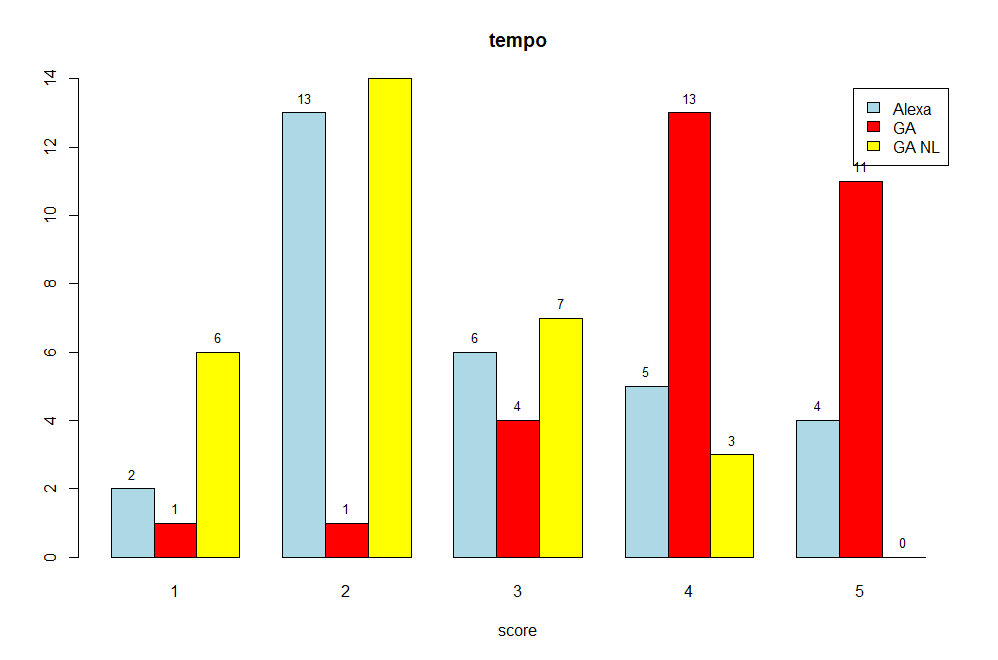
\includegraphics[width=0.9\linewidth]{../onderzoek/onderzoeksresultaten/vergelijking_assistenten_per_eigenschap/barplot/barplot_score_tempo}
    \caption{De score die de deelnemers hebben gegeven op het tempo van de assistenten}
    \label{fig:barplot-tempo}
\end{figure}

\begin{figure}[h]
    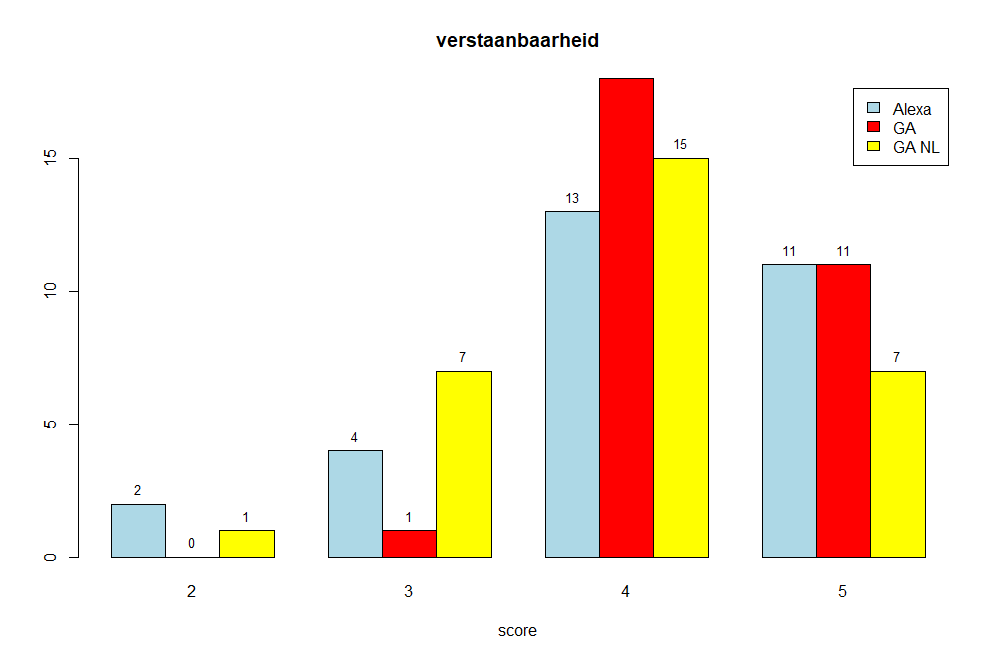
\includegraphics[width=0.9\linewidth]{../onderzoek/onderzoeksresultaten/vergelijking_assistenten_per_eigenschap/barplot/barplot_score_verstaanbaarheid}
    \caption{De score die de deelnemers hebben gegeven op de verstaanbaarheid van de assistenten}
    \label{fig:barplot-verstaanbaarheid}
\end{figure}

\begin{figure}[h]
    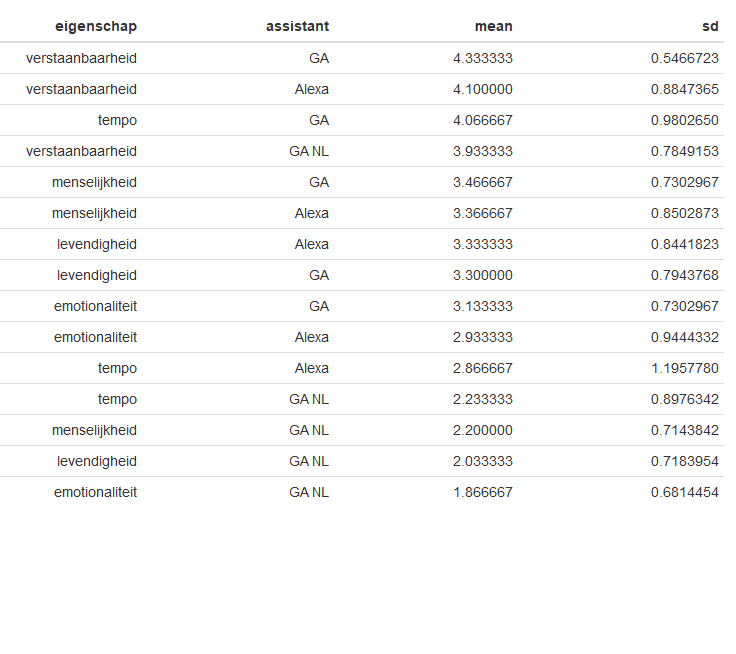
\includegraphics[width=0.9\linewidth]{../onderzoek/onderzoeksresultaten/vergelijking_assistenten_per_eigenschap/table_mean_sd_scores}
    \caption{De gemiddelde score en standaardafwijking van alle assistenten hun eigenschappen gesorteerd van hoog naar laag.}
    \label{fig:table-mean-sd-scores}
\end{figure}

Bij elke eigenschap is te zien hoe GA NL lager scoort dan GA en Alexa. Zelfs bij verstaanbaarheid, ondanks dat het Nederlands de moedertaal is van elke deelnemer. Het kan wel verklaren waarom het verschil in score tussen GA NL aan de ene kant en GA en Alexa aan de andere kant bij deze eigenschap het kleinste is. GA en Alexa, die beiden in het Engels opereren, scoren gelijkmatig op alle eigenschappen, behalve het tempo. Daar ligt het verschil tussen de drie assistent verdeeld en komt GA naar voren als de assistent met de hoogste score.
Twintig van de dertig deelnemers geven aan dat GA NL eerder klinkt als een robot, terwijl de helft vindt dat GA eerder klinkt als een mens. Ook al gaat het over dezelfde assistent, een verschil in taal zorgt voor heel wat kwaliteitsvermindering.
Emotionaliteit werd als enige eigenschap voor geen enkele assistent beoordeeld met de hoogste score. De verstaanbaarheid is de eigenschap met algemeen de hoogste score.
Levendigheid scoort hoog bij GA en Alexa, 25 van de 30 deelnemers gaven voor beide assistenten een score van 3 of meer.

Uit de waarnemingen van de staafdiagrammen en boxplots zijn enkele stellingen geschreven. Voor elke stelling is een t-test uitgevoerd om te bewijzen dat deze statistisch verantwoord of significant zijn. De p-waarde ligt bij elke test duidelijk onder het significantieniveau van 0.05, dus kunnen we steeds de nulhypothese verwerpen. De volgende stellingen zijn bewezen.
\begin{itemize}
    \item Alexa scoort hoger op emotionaliteit dan GA NL.
    \item GA scoort hoger op emotionaliteit dan GA NL.
    \item Alexa scoort hoger op levendigheid dan GA NL.
    \item GA scoort hoger op levendigheid dan GA NL.
    \item Alexa scoort hoger op menselijkheid dan GA NL.
    \item GA scoort hoger op menselijkheid dan GA NL.
    \item GA scoort hoger op tempo dan Alexa.
    \item Alexa scoort hoger op tempo dan GA NL.
    \item GA scoort hoger op verstaanbaarheid dan GA NL.
\end{itemize}

De resultaten van de uitgevoerde t-testen zijn te vinden onder de map onderzoek/onderzoeksresultaten in de repository beschreven in \ref{s:verwijzing naar repository}.

\subsection{Vergelijking van de eigenschappen per assistent}
\begin{figure}[h]
    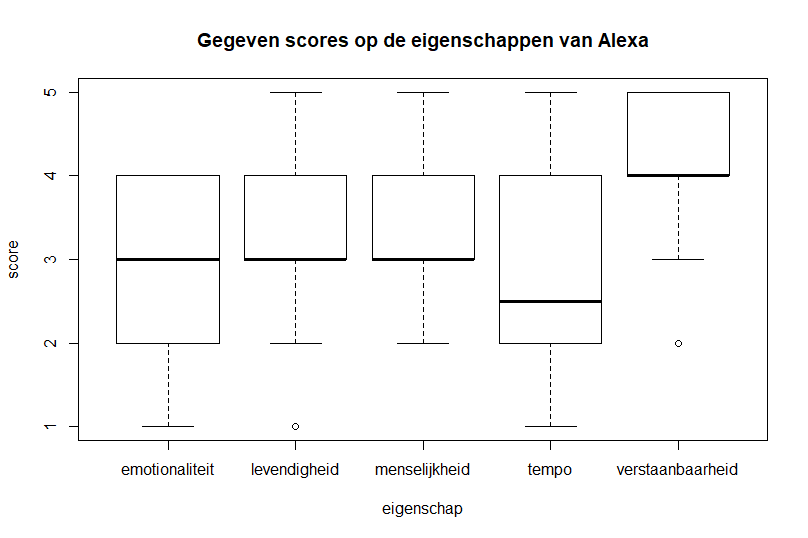
\includegraphics[width=0.9\linewidth]{../onderzoek/onderzoeksresultaten/vergelijking_eigenschappen_per_assistent/boxplot_score_eigenschappen_alexa}
    \caption{}
    \label{fig:boxplot-alexa}
\end{figure}

\begin{figure}[h]
    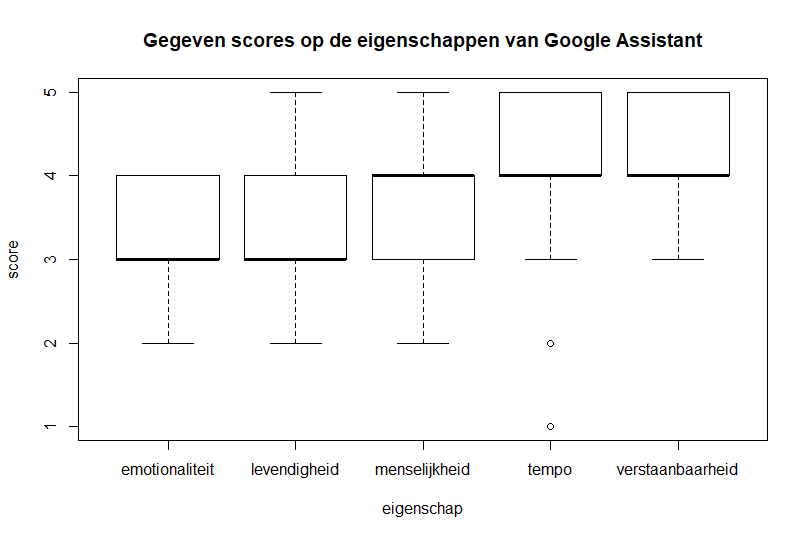
\includegraphics[width=0.9\linewidth]{../onderzoek/onderzoeksresultaten/vergelijking_eigenschappen_per_assistent/boxplot_score_eigenschappen_GA}
    \caption{}
    \label{fig:boxplot-ga}
\end{figure}

\begin{figure}[h]
    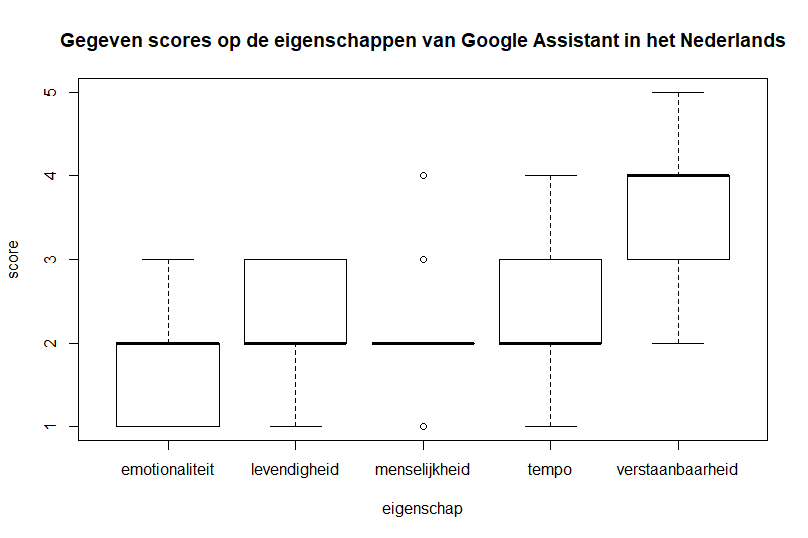
\includegraphics[width=0.9\linewidth]{../onderzoek/onderzoeksresultaten/vergelijking_eigenschappen_per_assistent/boxplot_score_eigenschappen_GA_NL}
    \caption{}
    \label{fig:boxplot-ganl}
\end{figure}

Door de gegeven boxplots kunnen we het onderlinge verschil tussen de eigenschappen van een assistent gaan bekijken. Alexa scoort van alle vijf de eigenschappen het laagst op tempo. Bij GA daarentegen hoort het tempo tot één van de betere eigenschappen. De gegeven scores voor het tempo van Alexa zijn het meest verspreid. 
Verstaanbaarheid scoort zowel bij Alexa als bij GA steeds een drie of hoger, op één uitschieter na.
GA krijgt voor geen enkele eigenschap de laagste score, op één uitschieter na.
GA NL scoort op emotionaliteit, levendigheid en menselijkheid nooit hoger dan een 2 of een 3, op 2 uitschieters na.

\section{Vergelijking van de assistenten in spraakherkenning}
\subsection{Een moeilijk te voeren onderzoek}
Alexa is er niet in geslaagd om de vraag 'someone fainted and now he is not breathing anymore' eens volledig te herkennen door naar de audiofragmenten te luisteren. Google Assistant is hier drie keer in geslaagd. Als de onderzoeker ter controle dezelfde vraag drie keer rechtstreeks stelt aan de assistenten, dan slagen ze er in om minstens 2 van de 3 keren de vraag volledig juist om te vormen naar tekst. Zo kan de opmerking gemaakt worden dat de assistenten slechter scoren op de opgenomen fragmenten dan op een vraag die rechtstreeks wordt gesteld. Hier is echter geen statistisch correct onderzoek naar gedaan.

Een andere bemerking bij het onderzoek is dat elke fout gelijk meetelt. Stel dat twee assistenten de uitspraak 'help me with a burn' omvormen naar tekst. De ene assistent begrijpt de vraag als 'help us for a burn' en de andere als 'tell me with a good'. Het voelt aan alsof de eerste assistent de vraag beter heeft begrepen dan de tweede, terwijl ze toch beide even veel fouten hebben gemaakt. de eerste assistent mist de woorden 'me' en 'with', de tweede assistent de woorden 'help' en 'burn'. Om de correctheid van een gevormde zin beter te interpreteren zou aan elk woord een soort hoofdzakelijkheid voor het begrijpen van de zin moeten toegekend worden. 'help' en 'burn' zijn sleutelwoorden om de zin te begrijpen. Er bestaan echter geen vaste regels om dit aan woorden toe te wijzen.

Als de onderzoeker merkt dat twee woorden verkeerd zijn omgevormd naar één woord, dan geldt de uitzondering dat dit telt als één fout. Een voorbeeld is 'for a whole day' dat wordt herkend door de assistent als 'for all day'. Deze interpretatie is echter niet objectief, waardoor de meting van het aantal fouten nog minder statistisch verantwoord is.

Ondanks dat er verschillende maatregelen zijn genomen om ervoor te zorgen dat elke assistent identiek dezelfde vraag krijgt, is deze opzet toch niet helemaal geslaagd. Alexa neemt elke conversatie op en bewaart ze in uw geschiedenis. Door enkele conversaties van tijdens het onderzoek te beluisteren is er opgemerkt dat hier en daar gekraak aanwezig is. Het gekraak was tijdens het onderzoek niet hoorbaar, waardoor de oorzaak waarschijnlijk bij de microfoon van de smartphone ligt. Het onderzoek is niet correct gevoerd omdat de sterkte van het gekraak kan variëren en mogelijks invloed heeft op de prestaties van de SST van een assistent. Een voorbeeld van een opgenomen interactie met Alexa, inclusief hoorbaar is te vinden onder onderzoek/onderzoeksresultaten/voorbeeld\_opgenomen\_vraag\_alexa in de repository beschreven in \ref{s:verwijzing naar repository}.
De onderzoeker heeft ook waargenomen dat de assistent bij het meermaals luisteren naar hetzelfde audiofragment steeds andere woorden heeft begrepen. Hier zijn geen geschreven resultaten van, maar bevestigen wel nog eens dat de beluisterde commando's variabel zijn.

Door de gegeven redenen is daarom beslist het aantal fouten tussen de assistenten niet te vergelijken. Uit de gevormde zinnen van de assistenten zijn wel enkele zaken vastgesteld.

\subsection{De gevormde zinnen}
\begin{figure}[h]
    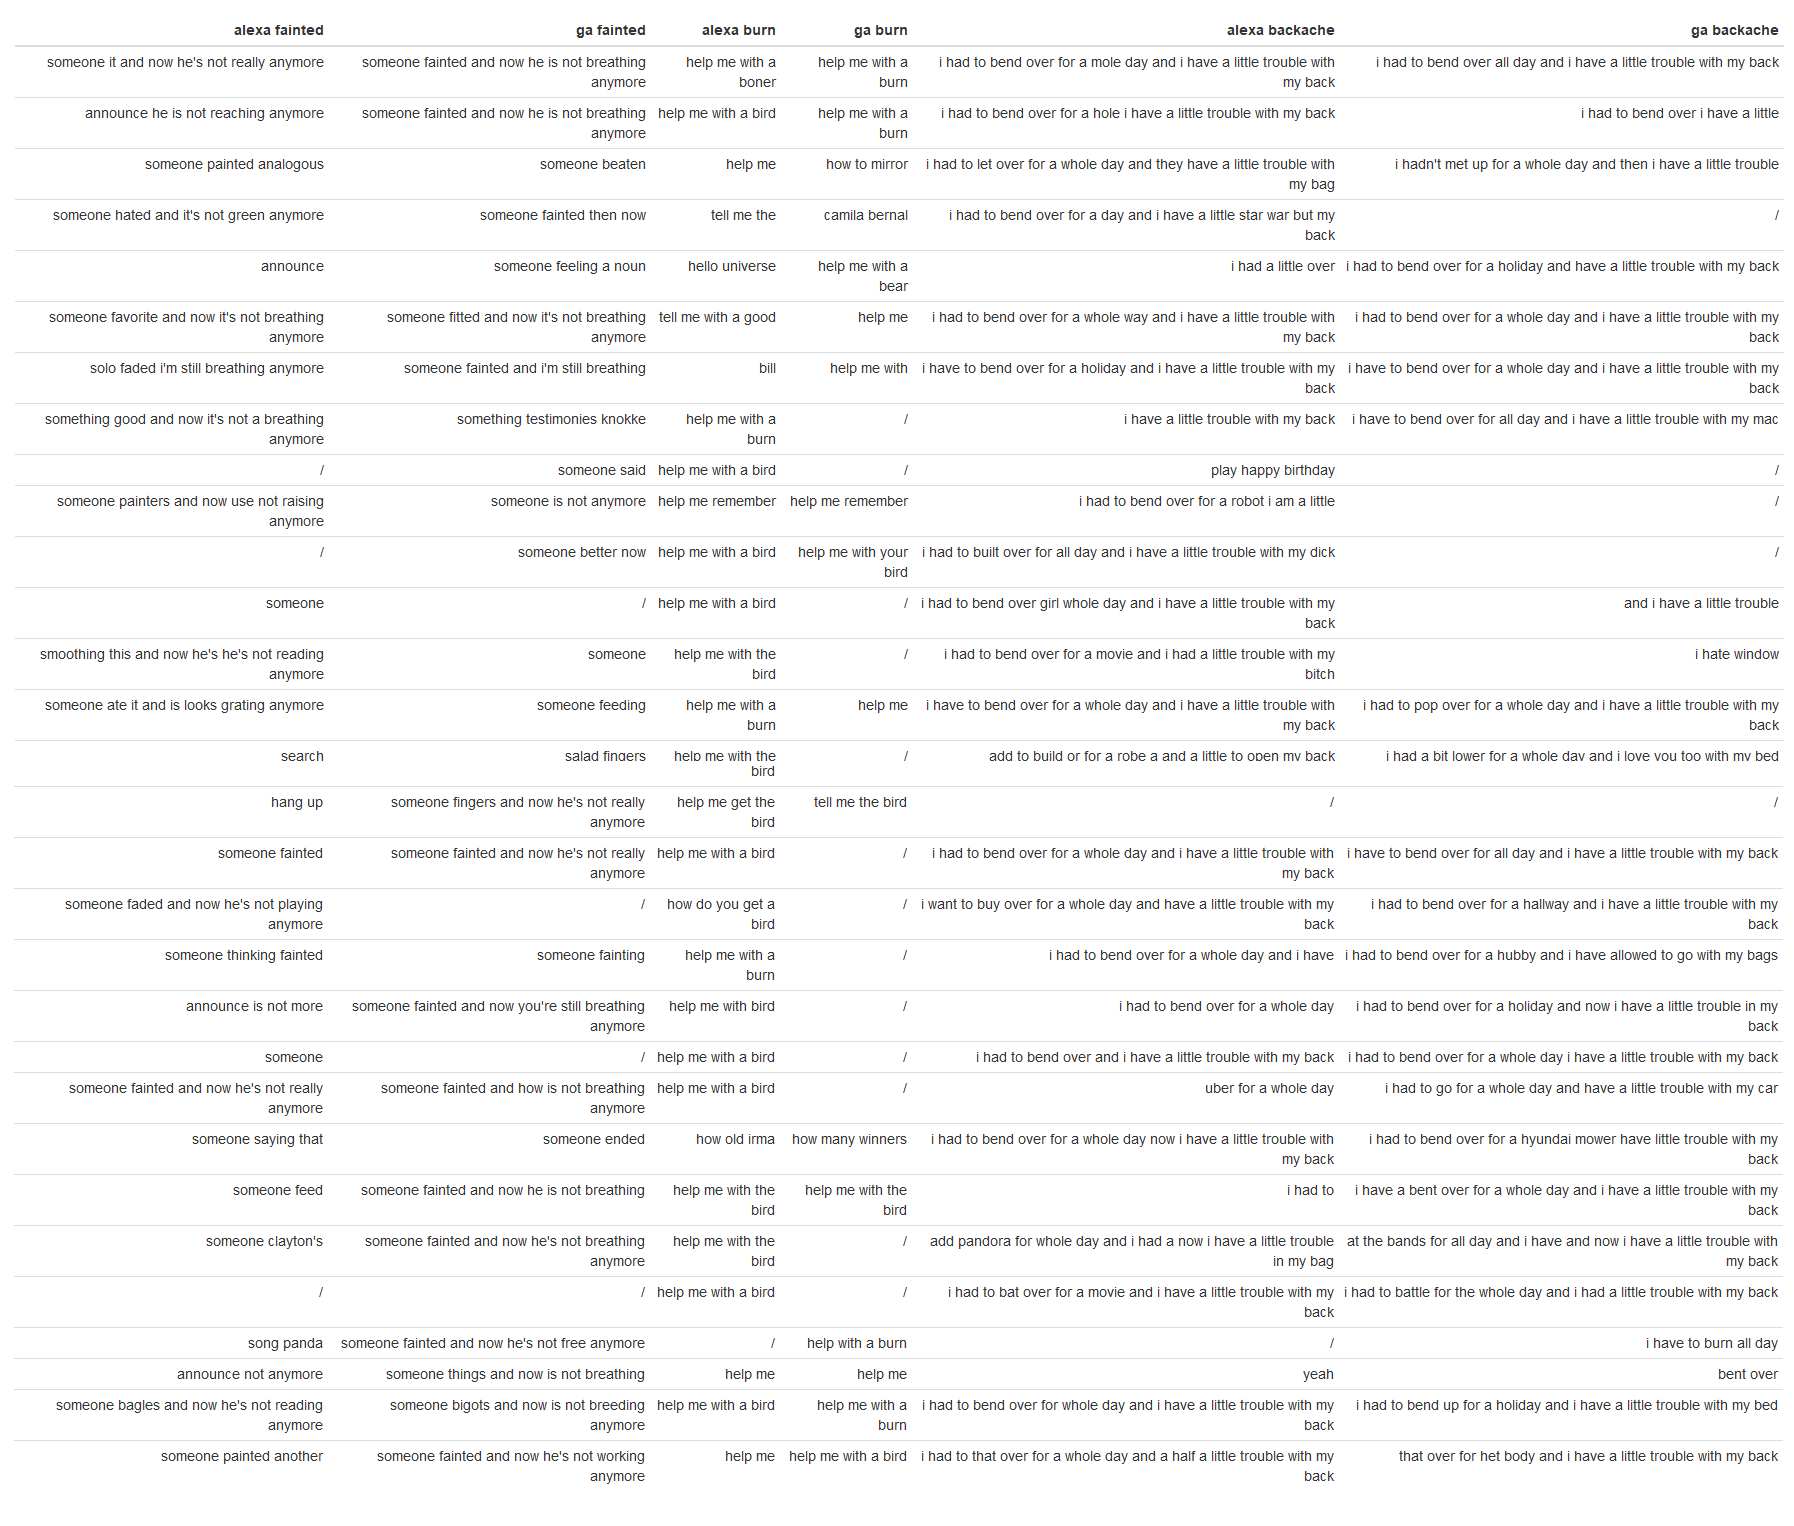
\includegraphics[width=1\linewidth]{../onderzoek/onderzoeksresultaten/vergelijking_tts_alle_teksten/tabel_alle_teksten}
    \caption{Een overzicht van de zinnen die de assistenten hebben begrepen uit de vragen van de deelnemers.}
    \label{fig:tabel-alle-teksten}
\end{figure}

Sommige opvallende zinnen uit de tabel zijn verder onderzocht. Enkele interessante fouten zijn gevonden.



 vb. and now he's -> announce
zou in dit onderzoek minder met vergelijking werken, maar met interessante misopvattingen


